% ************ Chapter 3 ************
%\renewcommand{\chaptername}{Chapter}
\chapter{Análise de Valor}
\label{cap:3}
%\emph{Este capitulo incide em apresentar de que forma as diferentes alternativas criam valor para o público alvo, e desta forma tirar conclusões sobre qual alternativa deve ser aprofundada}

O modelo a ser utilizado nesta secção será o Fuzzy Front End. Este processo de análise apresenta-se como mais adequado para projetos mais experimentais, dos quais não se tem uma definição concreta tanto da comercialização do mesmo, como a expetativas de retorno. Geralmente surge como incremento a um projeto já existente, pretendendo cobrir uma falha de negócio ou tecnológica.

Esta fase consiste no início do desenvolvimento de um produto. Esta passa pela identificação do problema e captação de ideias ou oportunidades. Por essa razão tem como característica uma maior incerteza sobre o que poderá vir a ser realizado, assim como qual será o público alvo.

A fase seguinte já requer que as ideias estejam bem estruturadas e os seus objetivos claros de modo a se realizar o desenvolvimento do produto.

Por fim, a comercialização é a última fase e consiste em definir detalhes como onde será introduzido o produto no mercado.

O modelo de New Concept Development Model é a representação das principais atividades do Fuzzy Front End. Este consiste em três componentes:

\begin{itemize}

\item Motor: Mecanismo que impulsiona as atividades de liderança e estratégia de negócio da organização;

\item Cinco Processos: São os processos que compõem o centro do modelo, que têm em conta a visão geral, a estratégia pretendida e a sua motivação;

\item Fatores de Influência: Variáveis não controláveis de origem interna ou externa ao projeto que afetam a sua inovação.

\end{itemize}

\begin{figure}[h]
    \begin{center}
    % Requires \usepackage{graphicx}
    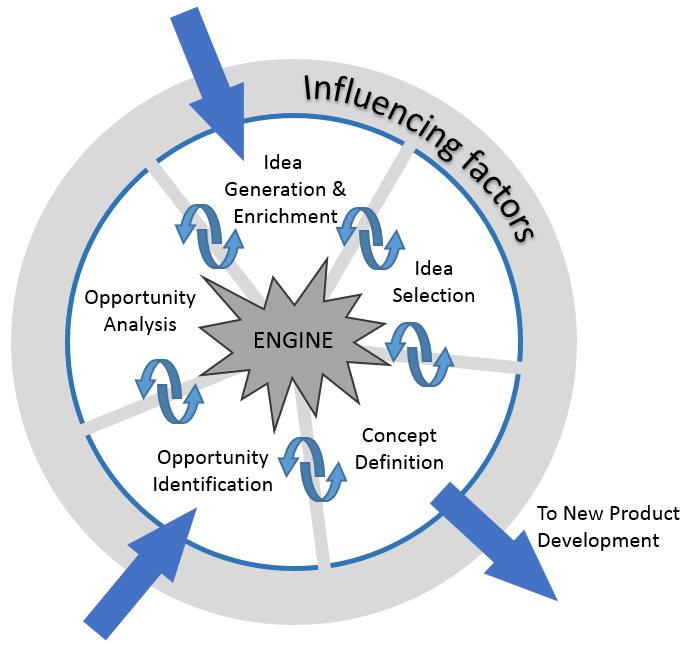
\includegraphics[width=0.5\textwidth]{figures/The-New-Concept-Development-NCD-model-Koen-et-al-2001.png}
    \caption{Representação New Concept Development Model}
    \end{center}
\end{figure}

\subsection{Identificação da Oportunidade}
A identificação da oportunidade é o input inicial para o modelo New Concept Development Model.
Neste contexto, a oportunidade surge no sentido de prevenir o acontecimento de escandalos como o conhecido Cambridge Analytica e outros "leaks" de informação que acontecem a um ritmo cada vez superior numa web baseada num paradigma que parece cada vez mais desajustado para a realidade que vivemos nos dias de hoje.

\subsection{Análise da Oportunidade}
O conceito "descentralização da web" não é novo, mas tem ganho ênfase nos últimos tempos e existem esforços notáveis para tornar este conceito numa realidade e tornar viável o surgimento de uma web mais livre e transparente.

Esta tese passa inicialmente por perceber que alternativas existem e qual pode ter mais potencial numa vertene de adoção massiva a médio prazo. Os seguintes projetos serão analisados:

\begin{itemize}

\item Solid - Solid é uma plataforma descentralizada para aplicações web. É baseada em RDF e tecnologias de web semantica. Para além disso providencia mecanismos de gestão de informação simples e ao mesmo tempo bastante potentes.\cite{solid_spec}

\item Blockstack - Um projeto open-source que ambiciona construir uma rede de computação descentralizada que proporcione uma alternativa full-stack à tradicional computação em cloud.\cite{blockstack_white_paper}

\item Diaspora - Um projeto baseado numa rede social descentralizada. O conceito consiste em permitir ao utilizador registar-se e guardar a sua informação no  "servidor" que pretender, podendo mesmo ser o seu próprio.\cite{diaspora_wiki}

\item Elastos - Projeto ambiciona proporcionar um novo paradigma de web baseado em tecnlogia blockchain. Este projeto tem duas grandes bandeiras: a proteção dos dados e a proteção dos direitos de autor.\cite{elastos_white_paper}

\end{itemize}

\subsection{Enriquecimento da ideia}
Esta fase consiste no aperfeiçoamento da ideia, incide no aperfeiçoamento da mesma até se estar contente e confiante na mesma.
Nesta fase é importante perceber os fatores que se apresentam como mais relevantes para uma framework capaz de potencializar um novo paradigma de web descentralizada:

\begin{itemize}
\item  Gestão de informação - No sentido de prevenir escândalos de acessos indevidos a informação pessoal e combater a monopolização dos dados, existe necessidade de garantir a defesa da sua propriedade. O facto de ser num contexto descentralizado, torna relevante perceber como poderão eventualmente ser acedidos os dados em diferentes contextos e aplicações

\item Mecanismo de autenticação e autorização - A propriedade dos dados é assegurada por mecanismos de autenticação e autorização. Este é ponto crucial e complexo, na medida em que terá de ser garantida para um de um determinado utilizador em qualquer aplicação, através dos mesmos dados.

\end{itemize}

\subsection{Seleção da ideia}
A seleção da ideia é o momento onde se assume qual o caminho que se pretende tomar com base nos processos anteriores.

Para esta componente foi utilizada a técnica AHP (analytic hierarchy proccess), esta técnica permite estruturar a a tomada de decisões complexas, contribuindo, desta forma, para que as conclusões sejam o mais acertadas possível.

\subsubsection{Critérios}

A primeira desta técnica é apresentar os critérios mais relevantes para a tomada de decisão.

\begin{table}[h]
\centering
\caption{Matriz Critérios}
\vspace{0.5cm}
\begin{tabular}{c|c|c|c} 
 - & Autenticação & Autorização & Armazenamento \\
\hline                          
Autenticação & 1 & 1 1/2 & 1,75 \\
Autorização &  2/3 & 1 & 1 1/4  \\
Armazenamento &  4/7 & 4/5 & 1 \\
Soma & 2 5/21 & 3 3/10 & 4 \\
\end{tabular}
\label{tab:ex_map}
\end{table}

\begin{table}[h]
\centering
\caption{Matriz Critérios Normalizada}
\vspace{0.5cm}
\begin{tabular}{c|c|c|c|c} 
 - & Autenticação & Autorização & Armazenamento & Média Ponderada \\
\hline                               
Autenticação & 21/47 & 5/11 & 7/16 & 45\% \\
Autorização &  14/47 & 10/33 & 5/16 & 30\% \\
Armazenamento &  12/47 &  8/33 & 1/4 & 25\% \\
Soma & 1 & 1 & 1 & 100\% \\
\end{tabular}
\label{tab:ex_map}
\end{table}

\pagebreak

\subsubsection{Prioridades Relativas}
Após os critérios estarem e as devidas prioridades estarem devidamente apresentadas, segue-se a apresentação e das diferentes alternativas, bem como a sua prestação face aos diferentes critérios.

\textbf{Autenticação}

\begin{table}[h]
\centering
\caption{Prioridades Relativas Autenticação}
\vspace{0.5cm}
\begin{tabular}{c|c|c|c|c|c} 
 - & Solid & BlockStack & Diaspora & Elastos & Prioridade Relativa \\
\hline                               
Solid & 41\% &	48\% &	44\% & 33\% \\
BlockStack &  21\% & 24\% &	22\% &	33\% &	25\% \\
Diaspora &  10\% &	12\% &	11\% & 11\%	& 11\% \\
Elastos & 28\% & 16\% & 22\% & 22\% & 22\% \\
\end{tabular}
\label{tab:ex_map}
\end{table}

\textbf{Autorização}

\begin{table}[h]
\centering
\caption{Prioridades Relativas Autorização}
\vspace{0.5cm}
\begin{tabular}{c|c|c|c|c|c} 
 - & Solid & BlockStack & Diaspora & Elastos & Prioridade Relativa \\
\hline                               
Solid & 26\% &	35\% &	10\% & 45\% & 29\% \\
BlockStack &  18\% & 25\% & 32\% & 21\% & 24\% \\
Diaspora &  43\% &	13\% &	17\% &	10\% & 20\% \\
Elastos & 13\% & 28\% &	42\% & 24\% & 27\% \\
\end{tabular}
\label{tab:ex_map}
\end{table}

\pagebreak

\textbf{Armazenamento}

\begin{table}[h]
\centering
\caption{Prioridades Relativas Armazenamento}
\vspace{0.5cm}
\begin{tabular}{c|c|c|c|c|c} 
 - & Solid & BlockStack & Diaspora & Elastos & Prioridade Relativa \\
\hline                               
Solid & 23\% & 35\% & 8\% & 44\% & 28\% \\
BlockStack &  17\% & 25\%	& 32\%	& 22\%	& 24\% \\
Diaspora &  47\% &	13\% & 17\%	& 10\% & 22\% \\
Elastos & 13\% & 28\% & 42\% & 24\% & 27\% \\
\end{tabular}
\label{tab:ex_map}
\end{table}

\subsubsection{Resultados}

\begin{table}[h]
\centering
\caption{Resultados AHP}
\vspace{0.5cm}
\begin{tabular}{c|c|c|c|c|c} 
 - & Autenticação & Autorização & Armazenamento & Valor Final & \\
\hline                               
Solid & 42\% &	29\% & 28\%	& 33\% & \\
BlockStack &  25\% & 24\% & 24\% & 24\% & \\
Diaspora &  11\% &	20\% & 22\% & 18\% & \\
Elastos & 22\% & 27\% & 27\% & 25\% & \\
\end{tabular}
\label{tab:ex_map}
\end{table}


Tendo em conta os estudos apresentados anteriormente, o caminho a seguir será aprofundar a framework Solid de forma a torná-la mais escalável e preparada para a uma possível adoção massiva.

\subsection{Definição do Conceito}
O momento da definição do conceito corresponde à fase final da formalização da ideia já escolhida anteriormente.

O conceito introduzido pelo Solid, em conjunto com o possível potencial de escalabilidade, permite tonar uma realidade o conceito de "Web Descentralizada"

\section{Proposta de Valor}
A proposta de valor representa o estudo da forma como os benefícios do produto poderão ter impacto para os clientes. Neste contexto o estudo deverá centrar-se em como esta framework poderá ter impacto na construção de uma web descentralizada.

\subsection{Modelo Fast}
Este modelo permite, de forma esquematizada, representar o a funcionalidade do sistema, baseando em pensamento crítico.

\begin{figure}[h]
    \begin{center}
    % Requires \usepackage{graphicx}
    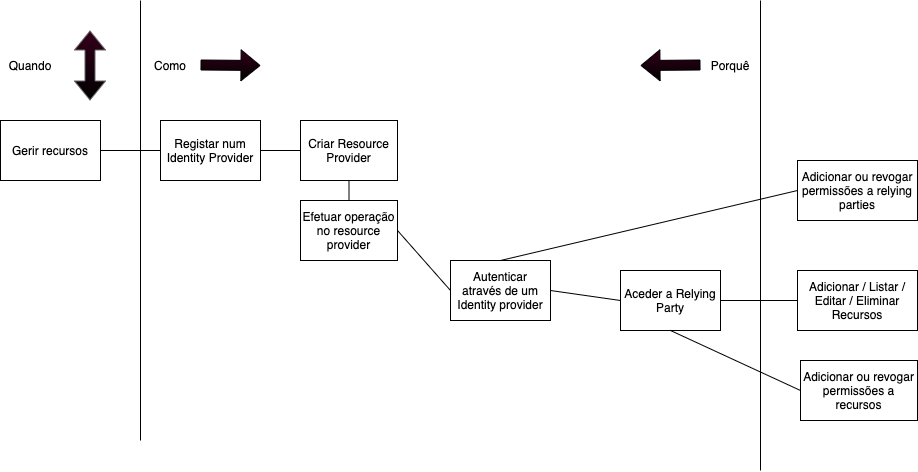
\includegraphics[width=1\textwidth]{figures/Canvas-FAST.png}
    \caption{Modelo Fast}
    \end{center}
\end{figure}

Este modelo permite perceber que o "core" de toda framework é os dados dos utilizador. Essa é a grande falha do modelo actual de web, modelo este que torna a informação infinitamente redundante e a expropria do utilizador.
Um novo paradigma deve garantir que os dados estão sob alçada do seu utilizador, podendo o mesmo a qualquer momento tomar ações como revogar acesso a determinadas aplicações (relying parties)

\section{Modelo Canvas}
\begin{figure}[h]
    \begin{center}
    % Requires \usepackage{graphicx}
    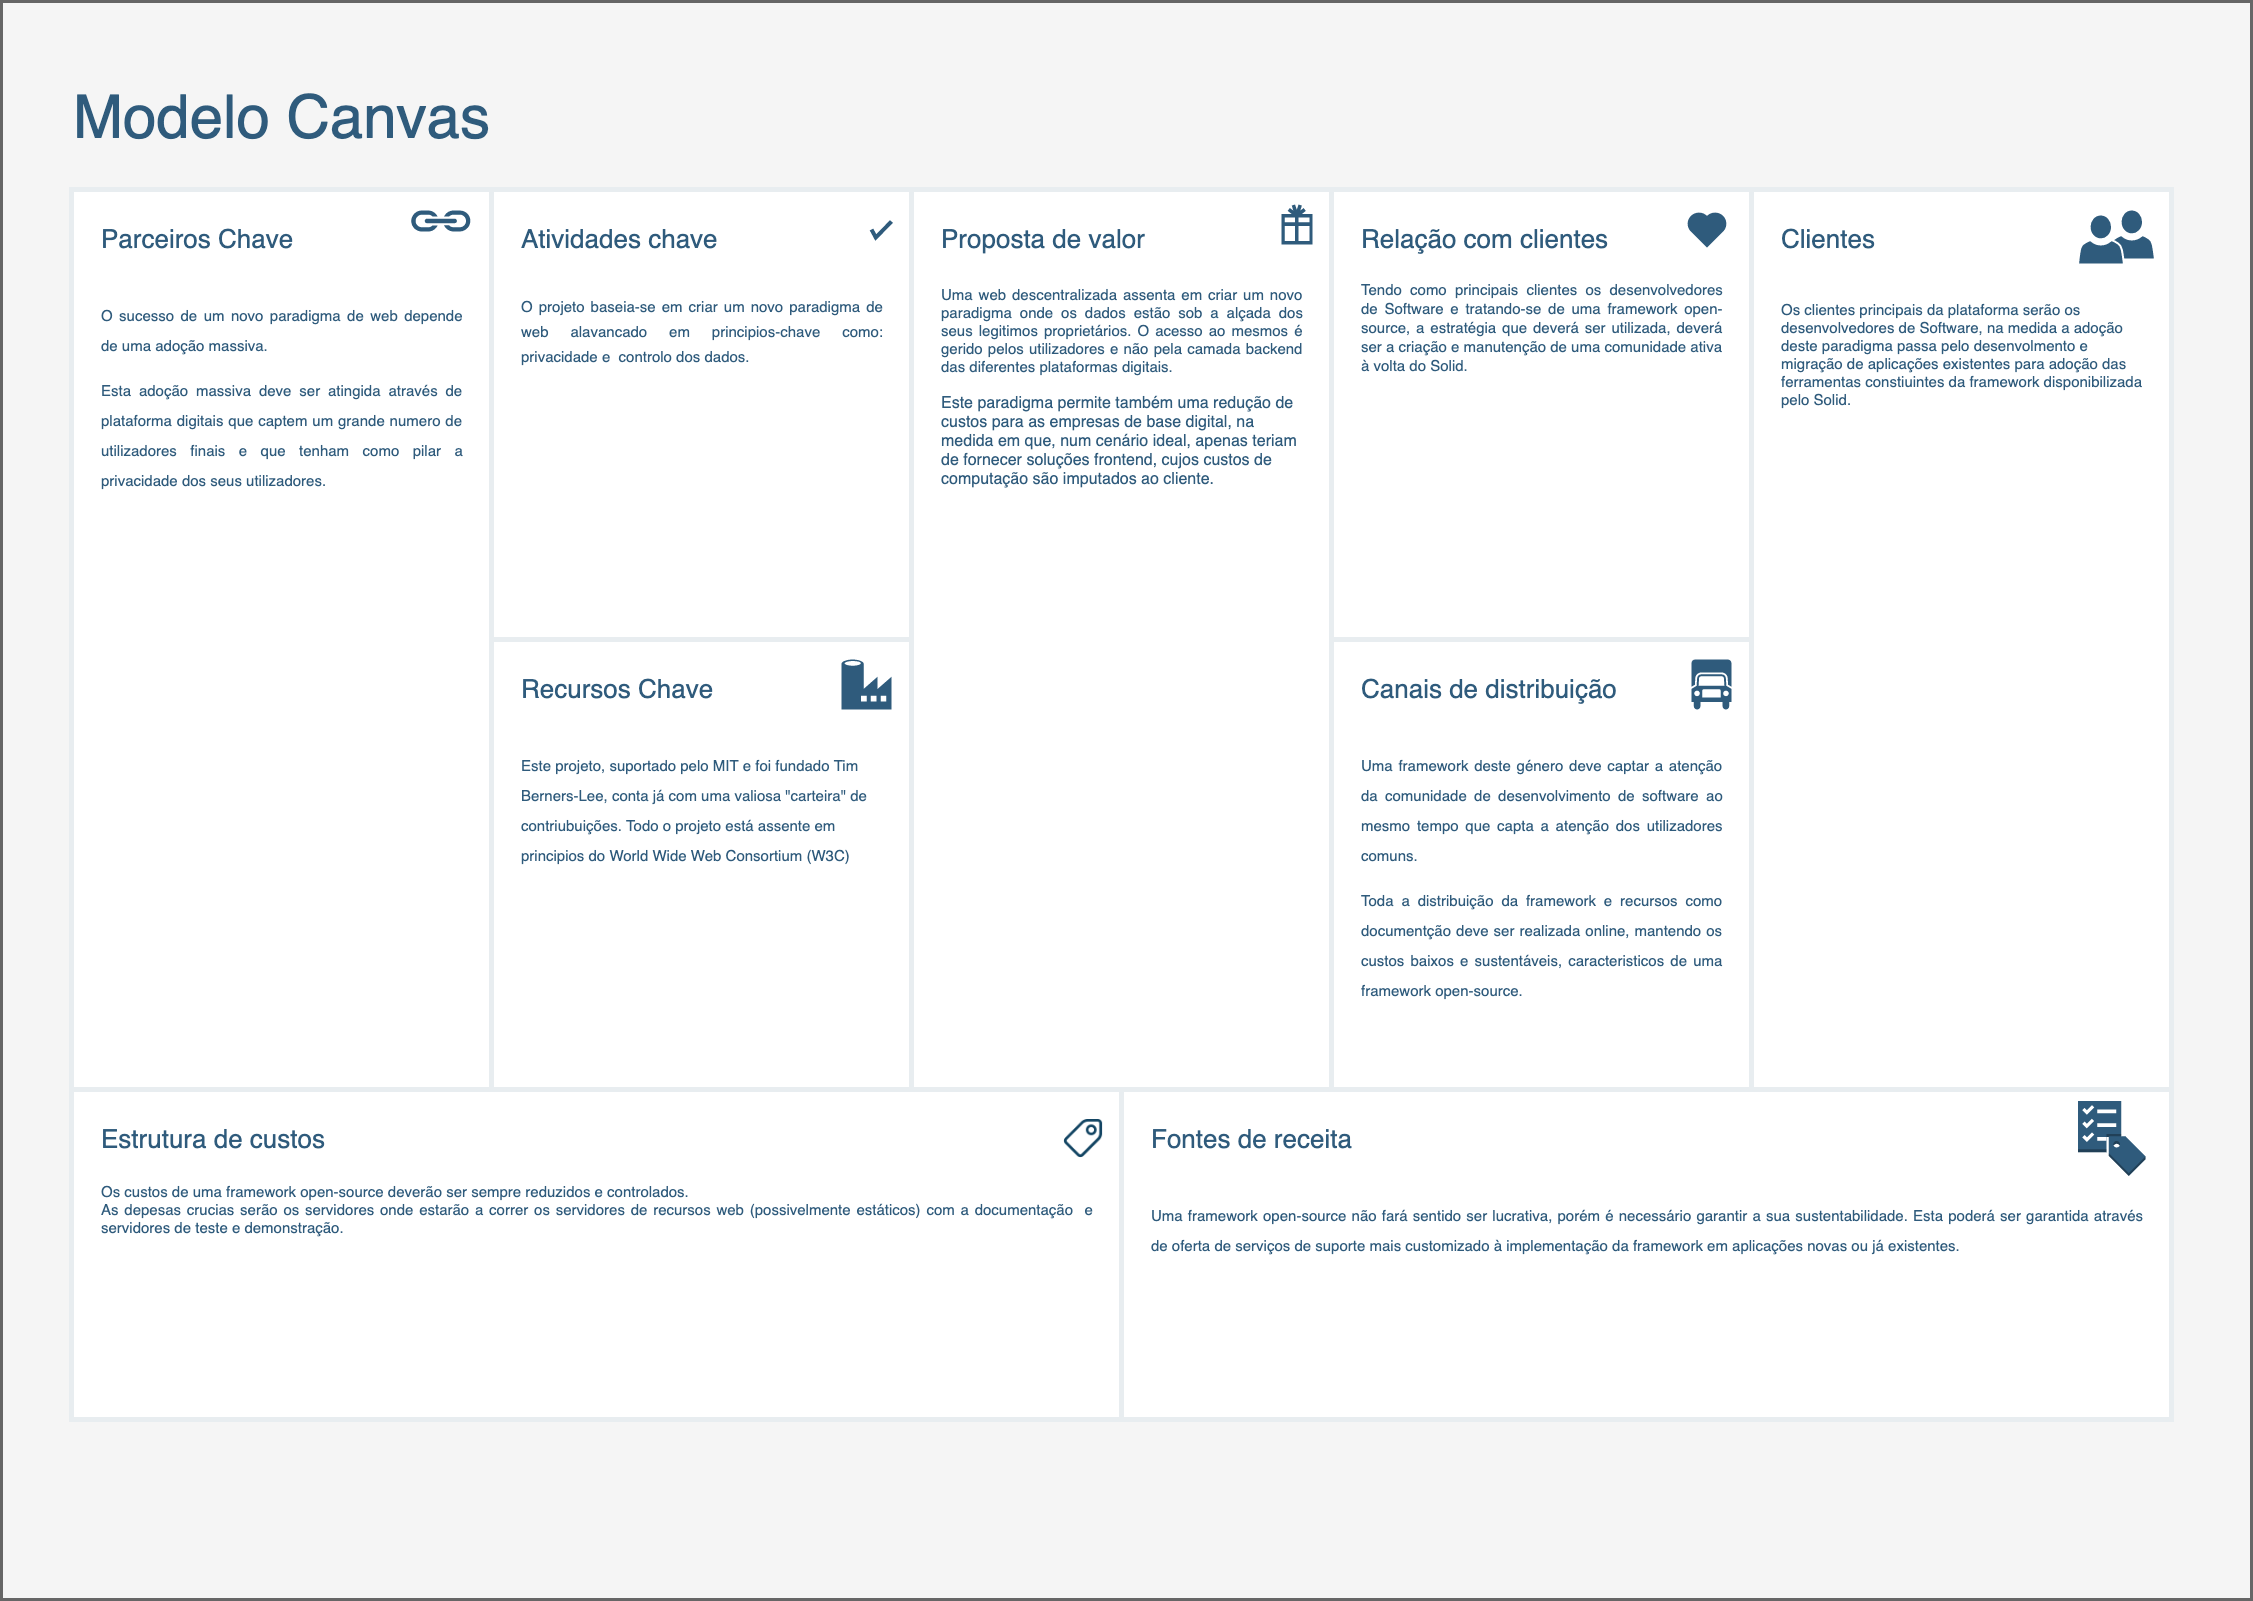
\includegraphics[width=1 \textwidth, angle=-90]{figures/Canvas-Canvas.png}
    \caption{Modelo Canvas}
    \end{center}
\end{figure}
